\documentclass[a4j,10pt]{jarticle}

\topmargin -17mm
\oddsidemargin -5mm
\textwidth 175mm
\textheight 260mm
\columnsep 8.6mm

\usepackage{epsf}
\usepackage{latexsym}
\usepackage{ascmac}
%\usepackage{graphicx}
\usepackage{multirow}
\usepackage{amsmath}
\usepackage{amsfonts}
\usepackage{multicol}
\usepackage{fancybox}
%\usepackage{theorem}
\usepackage{slashbox}
\usepackage[dvipdfm]{graphicx,color}
\usepackage{comment}
\usepackage{setspace}


\newtheorem{dfn}{定義}
\newtheorem{prof}{証明}
\newtheorem{theo}{定理}
\newtheorem{lemm}{補題}
\newtheorem{colo}{系}
\newcommand{\qed}{\hfill \hbox {\rule{6pt}{6pt}}}
\newcommand{\alb}{\allowbreak}

\newcommand{\TAB}{\hspace*{3mm}}
\newcommand{\IF}{\bf{if}}
\newcommand{\DO}{\bf{do}}
\newcommand{\ALL}{\bf{forall}}
\newcommand{\BEGIN}{\bf{begin}}
\newcommand{\WHILE}{\bf{while}}
\newcommand{\END}{\bf{end}}
\newcommand{\THEN}{\bf{then}}
\newcommand{\ELSE}{\bf{else}}
\newcommand{\UPON}{\bf{Upon}}
\newcommand{\INT}{\bf{int}}
\newcommand{\TIL}{\bf{until}}
\newcommand{\hp}{\hspace*{1zw}}

\newcommand{\ot}{\ensuremath{\leftarrow}}
\newcommand{\Scomment}[1]{\ensuremath{/\ast} #1 \ensuremath{\ast/}}
\newcommand{\BotN}{\ensuremath{\perp^n}}
\newcommand{\Vn}{\ensuremath{\mathcal{V}^n}}

\renewcommand{\thefootnote}{\arabic{footnote}}

\newcommand{\Omit}[1]{}

\newcounter{Codeline}
\newcommand{\Newcodeline}{\setcounter{Codeline}{1}}
\newcommand{\Cl}{{\theCodeline}: \addtocounter{Codeline}{1}}
\newcommand{\crm}{\\[-3.0mm]}

\renewcommand{\baselinestretch}{0.95}
\makeatletter  % --- 「おまじないモード」に入る

\renewenvironment{itemize}%  
{%
   \begin{list}{\parbox{1zw}{$\bullet$}}% 見出し記号/直後の空白を調節
   {%
      \setlength{\topsep}{1mm}
      \setlength{\itemindent}{0zw}
      \setlength{\leftmargin}{2zw}%  左のインデント
      \setlength{\rightmargin}{0zw}% 右のインデント
      \setlength{\labelsep}{0zw}%    黒丸と説明文の間
      \setlength{\labelwidth}{3zw}%  ラベルの幅
      \setlength{\itemsep}{0em}%     項目ごとの改行幅
      \setlength{\parsep}{0em}%      段落での改行幅
      \setlength{\listparindent}{0zw}% 段落での一字下り
   }
}{%
   \end{list}%
}

\renewenvironment{enumerate}
  {\ifnum \@enumdepth >3\relax\@toodeep\else
   \advance\@enumdepth\@
   \edef\@enumctr{enum\romannumeral\the\@enumdepth}%
   \list{\csname label\@enumctr\endcsname}{%
    \topsep\z@\parsep\z@\partopsep\z@\itemsep\z@
    \labelwidth1zw \labelsep1zw \listparindent1zw
    \itemindent1zw
    \clubpenalty-20
    \usecounter{\@enumctr}%
    \def\makelabel##1{\hss\llap{##1}}}%
   \fi}{\endlist}

\def\eqnarray{%
  \stepcounter{equation}%
  \def\@currentlabel{\p@equation\theequation}%
  \global\@eqnswtrue
  \m@th
  \global\@eqcnt\z@
  \tabskip\@centering
  \let\\\@eqncr
  $$\everycr{}\halign to\displaywidth\bgroup
    \hskip\@centering$\displaystyle\tabskip\z@skip{##}$\@eqnsel
    &\global\@eqcnt\@ne \hfil${{}##{}}$\hfil
    &\global\@eqcnt\tw@ $\displaystyle{##}$\hfil\tabskip\@centering
    &\global\@eqcnt\thr@@ \hb@xt@\z@\bgroup\hss##\egroup
  \tabskip\z@skip\cr}
  
%\renewcommand{\section}{%
%   \@startsection{section}{1}{\z@}%
%   {0.4\Cvs \@plus.0\Cdp \@minus.2\Cdp}%  上の空き
%   {0.2\Cvs \@plus.1\Cdp \@minus.3\Cdp}%  下の空き
%   {\reset@font\normalsize\bfseries}}%         字の大きさ
%
%\renewcommand{\subsection}{%
%   \@startsection{subsection}{1}{\z@}%
%   {0.4\Cvs \@plus.0\Cdp \@minus.2\Cdp}%  上の空き
%   {0.2\Cvs \@plus.1\Cdp \@minus.3\Cdp}%  下の空き
%   {\reset@font\normalsize\bfseries}}%         字の大きさ
%
%\renewcommand{\subsubsection}{%
%   \@startsection{subsection}{1}{\z@}%
%   {0.4\Cvs \@plus.0\Cdp \@minus.2\Cdp}%  上の空き
%   {0.2\Cvs \@plus.1\Cdp \@minus.3\Cdp}%  下の空き
%   {\reset@font\normalsize\bfseries}}%         字の大きさ
%
%\renewcommand{\paragraph}{%
%   \@startsection{paragraph}{4}{\z@}
%   {1.0ex plus 1ex minus .2ex}
%   {-1em}{\normalsize\bf}}

\floatsep 2pt plus 2pt minus 2pt
\textfloatsep 5pt plus 2pt minus 2pt

\makeatother   % --- 「おまじないモード」から抜ける
%$
\begin{document}
%ページ番号なし
\pagestyle{empty}
\twocolumn[
\vspace{-5mm}
\begin{center}
{\Large 無線センサネットワークにおけるベースステーションからの\\無線波情報を利用した負荷分散動的ルーティングアルゴリズム}\\

\vspace*{2mm}
{\large 渡部連太郎 角川裕次 増澤利光}\\
大阪大学 大学院情報科学研究科 コンピュータサイエンス専攻\\
\end{center}

{\small
\begin{spacing}{0.85}
%あぶすと
{\bf 概要}
 多数の安価な小型無線装置内蔵センサが相互にマルチホップ通信を行うことで構成される無線センサネットワークは,その適用分野の広さから様々なアプリケーションに利用されている.無線センサネットワークにおいてはセンサ間での消費電力を平均化し,ネットワークの存続時間を延ばすことが重要である.本研究は各センサノードが残存電力やセンシング情報収集施設からの距離を考慮した上で,メッセージの送信先を確率的に決定する手法の考案を目的とする.本稿ではその手法の概要を説明し,予備実験により手法の妥当性を簡易に検証した結果を示す.
\end{spacing}
}
\vspace{6mm}
]
%\keyword{
% キーワード
%}

%\toc
 % これは目次用


%%%%%%%%%%%%%%%%%%%%%%%%%%%%%%%%%%%%%%%%%%%%%%%%%%%%%%%%%%%%%%%%%%%%%%%%
\section{はじめに}
無線センサネットワーク(WSNs)とは,多数の安価な小型無線装置内蔵センサ(ノード)をフィールドに配置し,ノードがセンシングにより得た情報を収集施設(ベースステーション)へ転送することでフィールド全体の情報を収集するネットワークである.WSNsは対象の追跡や環境モニタリングなど様々なアプリケーションに利用され,その適用分野の広さから大きく期待されている.WSNsにおいてセンサは電池駆動である場合が多く,使用電力に制限がある.よってネットワークの存続時間を高めるために各ノードの消費電力を抑え,かつノード間での消費電力を平均化することが重要である.各ノードは通信可能距離内のノードと相互に通信することが可能であり,取得した情報はマルチホップ通信によりベースステーションに集められる.このようなネットワークの性質上,ベースステーションに近いノードほどデータ転送を行う頻度が高いため,消費電力が非均一となりネットワークの存続時間を短くする原因となる可能性が高い.そこでネットワークの存続時間を延ばすため,ノードの残存電力やベースステーションからの距離によって適切なメッセージ転送経路を決定的に計算する手法が考案されている.

本研究では,各ノードが残存電力やベースステーションからの距離を考慮した上で,メッセージの送信先を確率的に決定する手法の考案を目的とする.本手法では各ノードが確率的かつ局所的にメッセージの送信先を決定することで,特定のノードで大量のメッセージが生成される場合にも高確率で負荷を分散し,ネットワーク存続時間を延ばすことが可能である.またネットワーク内のどのベースステーションやノードもメッセージの転送経路全体を把握せず動作するため,頑健性が高く,適用するアプリケーションのセキュリティ面での安全性向上を見込むことができる.

本稿では提案手法の概要と,手法の妥当性を簡易に検証する予備実験の結果を紹介する.


% マルチホップ通信

%%%%%%%%%%%%%%%%%%%%%%%%%%%%%%%%%%%%%%%%%%%%%%%%%%%%%%%%%%%%%%%%%%%%%%%%

\section{諸定義}
WSNsのネットワークやアーキテクチャのモデルは,適用するアプリケーションに応じて様々なものが用いられる.本稿で提案する手法と予備実験においては以下のモデルを定義する.

\subsection{ネットワークモデル}

\subsubsection{センサノード}
全てのセンサノード(以降ノード)の初期配置はランダムで大局的に一意なIDは割り当てられない.センシング可能領域は自身から半径$R_s$以内,他ノードとの通信可能領域は$R_c(\le R_s)$以内とする.またノードは初期配置から移動せず,フィールドにおける自身の座標を認識するGPSなどの機能は保有していないと仮定する.

\subsubsection{ベースステーション}
ランダムに配置された,フィールドに1つのベースステーションを仮定する.ベースステーションには安定して電力が供給される.またネットワーク全体に到達する強力な電波を発信することが可能なである.

\subsection{電力消費モデル}
以下の電力消費モデルを仮定する.\par
\vspace{2mm}
 \hspace{6mm} 送信時 : \hspace{3mm} $E_{Tx}(l,d)=lE_{elec}+l \varepsilon_{fs}d^2$ \par
 \hspace{6mm} 受信時 : \hspace{3mm} $E_{Rx}(l)=lE_{elec}$ \par
\vspace{2mm}
$l$をメッセージのbit長,$d$を送受信するノード間の距離とする.$E_{elec}$は信号の符号化方式や振幅,フィルタ方式などに基づく係数である.$\varepsilon_{fs}$は信号増幅器の電力消費に関わる係数である.


% ネットワークモデル
% ノード
% ベースステーション
% 電力消費モデル

%%%%%%%%%%%%%%%%%%%%%%%%%%%%%%%%%%%%%%%%%%%%%%%%%%%%%%%%%%%%%%%%%%%%%%%%








\section{提案手法の概要}
本章では,各ノードがメッセージの転送先をベースステーションからのホップ数と隣接ノードの残存電力,隣接ノードとの距離に基づいて確率的に決定する手法を提案する.メッセージの転送経路が確率的に変化することで,特にメッセージが特定のエリアで大量に発生する場合に,特定の経路上のノードの集中的な電力消費を緩和することができる.本手法は各ノードが自身と各隣接ノードの,ベースステーションからのホップ数を知っていることを仮定している.
ノード$i$の隣接ノード集合を$\mathbb{N}_i$,ベースステーションからのホップ数を$d_i$とする.各ノード$i$はベースステーションからのホップ数によって隣接ノード集合を以下の$\mathbb{L}_{d_i-1},\mathbb{L}_{d_i},\mathbb{L}_{d_i+1}$へ分割し,それぞれへの送信確率を設定する.
\begin{eqnarray*}
& \mathbb{L}_{d_i-1} & = \{j \in \mathbb{N}_i | d_{j} = d_{i}-1 \} \\
& \mathbb{L}_{d_i} & = \{j \in \mathbb{N}_i | d_{j} = d_{i} \} \\
& \mathbb{L}_{d_i+1} & = \{j \in \mathbb{N}_i | d_{j} = d_{i}+1 \}
\end{eqnarray*}
ノード$i$はメッセージ送信時,設定された確率に基づき送信する隣接ノード集合を決定する.決定したノード集合中に複数のノードが存在する場合,自身とそれらのノードの距離と残存電力に基づき,送信先のノードを1つ決定する.

%%%%%%%%%%%%%%%%%%%%%%%%%%%%%%%%%%%%%%%%%%%%%%%%%%%%%%%%%%%%%%%%%%%%%%%%

\section{予備実験}
メッセージが特定のエリアで集中的に発生した場合,必ずしもメッセージがベースステーションへ近づかないような転送をすることで,ネットワークの存続時間が延びることをシミュレーション実験により検証した.
提案手法と比較手法において,各ノードはベースステーションからのホップ数に基づき,メッセージの送信先となる隣接ノード集合を選択する.このとき選択したノード集合が空集合ならばそのメッセージは消失する.アルゴリズム開始から消失したメッセージの合計数が一定値$LL$を越えるまでのラウンド数をネットワーク存続時間とみなし,各アルゴリズムを評価する.

\subsection{各種定義}
今回の実験では簡単のため,ノードがメッセージを送信する隣接ノード集合を決定した後,複数の送信先ノード候補が存在した場合,それらとの距離やそれらの残存電力に依存しない一様ランダムな送信先ノードの選択を行う.またメッセージはランダムに選択されたノードで$I$回連続で発生するとする.


\subsubsection{比較手法}
提案手法と比較する手法は,各ノードが必ずベースステーションへ近づくようにメッセージを送信する手法を用いる.ノードはメッセージを送信する際,自身よりベースステーションからのホップ数が小さい隣接ノード集合を選択する.複数のノードが含まれる場合は,提案手法と同様,一様ランダムにその中から1つのノードを選択する.

\newpage
\subsubsection{確率設定}
メッセージ送信時に利用する確率の設定について説明する.
ノード$i$が,ベースステーションからのホップ数が$h ( d_i-1 \le h \le d_i+1 )$であるノード集合$\mathbb{L}_{h}$のいずれかにメッセージを送信する確率を$P(d_i,h)$とする.
今回は,ノード$i$が送信したメッセージがベースステーションへ到達するまでに転送回数の期待値が$kd_i$($k$はパラメータとして入力値を設定)となるように$P(d_i,d_i-1)$,$P(d_i,d_i)$,$P(d_i,d_i+1)$を設定する.具体的には以下の式を満たすよう,ランダムに設定する.提案手法については$k > 1$とする.
\begin{eqnarray*}
\frac{1}{k} \le P(d_i,d_i-1) \le \frac{1}{2} + \frac{1}{2k} \\
P(d_i,d_i) = 1 + \frac{1}{k} -2P(d_i,d_i-1) \\
P(d_i,d_i+1) = P(d_i,d_i-1) - \frac{1}{k}
\end{eqnarray*}
一方,比較手法においては必ずベースステーションへ近づくようにメッセージを送信するため,$k=1$として以下のように各確率を定めたものとみなすことができる.
\begin{eqnarray*}
& P(d_i,d_i-1) & = 1 \\
& P(d_i,d_i) & = 0 \\
& P(d_i,d_i+1) & = 0
\end{eqnarray*}


\subsubsection{パラメータ}
実験に使用する各種パラメータの設定値を表\ref{tab:parameter}に示す.

\vspace{5mm}
\begin{table}[htb]
  \begin{center}
    \begin{tabular}{cc} \hline
      パラメータ & 値 \\  \hline
      フィールドサイズ & ($100\times100$)m \\
      ノード数 & 100, 200 \\
      初期電力 & 2.0J \\
      $通信可能距離$ & 20m \\
      $k$ & 1.0, 2.0 ,...,10.0 \\
      $I$ & 10, 100, 1000 \\
      $E_{elec}$ & 50 nJ/bit \\
      $\varepsilon_{fs}$ & 10 pJ/bit/${\rm m^2}$ \\
      $l$ & 4000 bit \\
      $LL$ & 10000 \\ \hline
    \end{tabular}
    \caption{各種パラメータ値}
    \label{tab:parameter}
  \end{center}
\end{table}
\vspace{-7mm}

\newpage
\subsection{結果と考察}
メッセージがベースステーションへ到達するまでの転送回数期待値の係数$k$とメッセージ連続発生数$I$によるネットワーク存続時間の変化を記録した.ノード数が100の場合の結果を図\ref{graph:N100}に,200の場合の結果を図\ref{graph:N200}に示す.

\begin{figure}[h]
  \begin{center}
  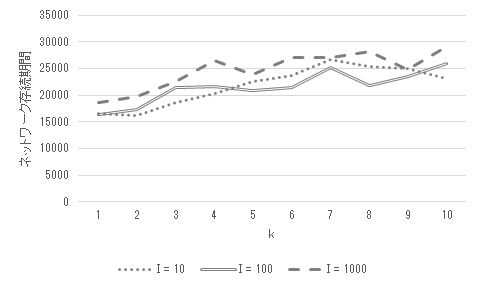
\includegraphics[width=8.5cm,clip]{./N100.png}
  \vspace{-8mm}
  \caption{ノード数100での結果}
  \label{graph:N100}
  \end{center}
\end{figure}

\begin{figure}[h]
  \begin{center}
  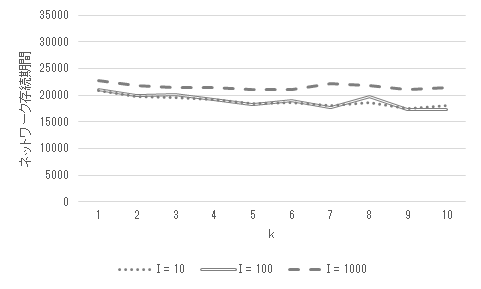
\includegraphics[width=8.5cm,clip]{./N200.png}
  \vspace{-8mm}
  \caption{ノード数200での結果}
  \label{graph:N200}
  \end{center}
\end{figure}

横軸$k$の値が1のデータが比較手法,2~10のデータが提案手法の結果を示している.

ノード数が100の場合,いずれの$I$についても,比較手法に対して提案手法の方がネットワーク存続時間が長くなり,かつ$k$が増加するにつれてネットワーク存続時間も長くなる傾向が見られる.
% ただし,グラフ全体をみてわかる通り,$k$の値を固定したとき$I$が小さいほどネットワーク存続時間が長くなるとは限らない

一方,ノード数が200の場合,$k$が増加させるにつれてネットワーク存続時間は緩やかに減少している.これはフィールドサイズに対してノード数が多くなったことで,グラフの半径が減少,ノードの平均次数が増加したために比較手法はネットワーク存続時間が増加,提案手法は強みが薄れネットワーク存続時間が減少したためと考えられる.

% \vspace{-1cm}

%%%%%%%%%%%%%%%%%%%%%%%%%%%%%%%%%%%%%%%%%%%%%%%%%%%%%%%%%%%%%%%%%%%%%%%%
\section{おわりに}
本稿では特定のノードで大量のメッセージが生成される場合に,一部のノードに負荷が集中することを回避することで,ネットワークの存続時間を延長する手法の概要を説明した.また予備実験により,特定のケースでは提案手法によりネットワークの存続時間が延長されることを検証した.しかし状況によっては存続時間が短くなる結果を示すケースもあるため,今後はノードの残存電力や自身との距離を考慮したメッセージ送信先の決定法を模索しつつ本手法の性質を詳細に検証する必要がある.さらに,複数のベースステーションへの対応や,強力な伝送波を送信することができるベースステーションの能力を活かした改良を行う予定である.

%%%%%%%%%%%%%%%%%%%%%%%%%%%%%%%%%%%%%%%%%%%%%%%%%%%%%%%%%%%%%%%%%%%%%%%%


\vspace{1cm}
\small
\begin{thebibliography}{9}

\bibitem{1}
Wendi B. Heinzelman, Anantha P. Chandrakasan and Hari Balakrishnan,“An Application-Specific Protocol Architecture for Wireless Microsensor Networks,”IEEE Transactions on Wireless Communications, Vol.1, No.4, pp.660-670, 2002.

\bibitem{2}
H. Zhou, D. Luo, Y. Gao and D. Zuo, "Modeling of Node Energy Consumption for Wireless Sensor Networks," Wireless Sensor Network, Vol.3 No.1, pp.18-23, 2011.

\bibitem{3}
Shashidhar Rao Gandham, Milind Dawande, Ravi Prakash and S. Venkatesan,“Energy Efficient Schemes for Wireless Sensor Networks with Multiple Mobile Base Stations,”in: Proc. IEEE Globecom 2003, San Francisco, CA December 1-5, vol.1, pp. 377-381, 2003.

\bibitem{4}
J. Cota-Ruiz, P. Rivas-Perea, E. Sifuentes and R. Gonzalez-Landaeta, "A Recursive Shortest Path Routing Algorithm With Application for Wireless Sensor Network Localization," in IEEE Sensors Journal, vol.16, no.11, pp.4631-4637, June, 2016.

\bibitem{5}
Fan Ye, A. Chen, Songwu Lu and Lixia Zhang, "A scalable solution to minimum cost forwarding in large sensor networks," Computer Communications and Networks, 2001. Proceedings. Tenth International Conference on, Scottsdale, pp.304-309, 2001.

\bibitem{6}
D. b. Zou and Y. B. Wang, "Adaptive energy-aware routing framework in transmission cost constrained wireless sensor networks," 2013 IEEE Global Communications Conference (GLOBECOM), Atlanta, GA, pp.534-538, 2013.

\bibitem{7}
P.B.Manoj and Sai Sandeep Baba, "Random Routing Algorithms for Wireless Sensor Networks," International Journal of Advanced Research in Computer and Communication Engineering, vol.1, issue 1, March, 2012.

\bibitem{8}
Zhixin Liu, Qingchao Zhenga, Liang Xuea and Xinping Guana, "A Distributed Energy-efficient Clustering Algorithm with Improved Coverage in Wireless Sensor Networks," Future Generation Computer Systems 28, vol.28, no.5, pp.780-790, May, 2012.

\bibitem{9}
Y. Liao, H. Qi and W. Li, "Load-Balanced Clustering Algorithm With Distributed Self-Organization for Wireless Sensor Networks," in IEEE Sensors Journal, vol.13, no.5, pp.1498-1506, May, 2013.

\end{thebibliography}

\small

\end{document}
